% ==============================================================================
% INFORME DE SUSTENTACIÓN - SISTEMA WEB DE MATRÍCULA UNIVERSITARIA
% Universidad Nacional Jorge Basadre Grohmann (UNJBG)
% ==============================================================================
\documentclass[12pt,a4paper]{article}

% --- Paquetes ---
\usepackage[utf8]{inputenc}
\usepackage[T1]{fontenc}
\usepackage[spanish,es-noshorthands]{babel}
\usepackage{geometry}
\usepackage{graphicx}
\usepackage{booktabs}
\usepackage{longtable}
\usepackage{array}
\usepackage{xcolor}
\usepackage{colortbl}
\usepackage{hyperref}
\usepackage{fancyhdr}
\usepackage{titlesec}
\usepackage{enumitem}
\usepackage{listings}
\usepackage{caption}
\usepackage{float}
\usepackage{amsmath}
\usepackage{lmodern}
\usepackage{microtype}
\usepackage{tcolorbox}
\usepackage{tabularx}
\usepackage{multirow}
\usepackage{pdfpages}

% --- Geometría ---
\geometry{
  top=2.5cm, bottom=2.5cm,
  left=2.5cm, right=2.5cm
}

% --- Colores corporativos ---
\definecolor{unjbgblue}{RGB}{0,51,102}
\definecolor{unjbgred}{RGB}{180,30,30}
\definecolor{lightgray}{RGB}{245,245,245}
\definecolor{darkgray}{RGB}{80,80,80}
\definecolor{codebg}{RGB}{250,250,250}
\definecolor{accent}{RGB}{0,120,212}

% --- Listings para SQL ---
\lstset{
  basicstyle=\small\ttfamily,
  backgroundcolor=\color{codebg},
  frame=single,
  rulecolor=\color{gray!40},
  breaklines=true,
  breakatwhitespace=true,
  tabsize=2,
  showstringspaces=false,
  keywordstyle=\bfseries\color{unjbgblue},
  commentstyle=\itshape\color{darkgray},
  stringstyle=\color{unjbgred},
  numbers=left,
  numberstyle=\tiny\color{gray},
  numbersep=6pt,
  xleftmargin=12pt,
  captionpos=b
}
\lstdefinelanguage{SQL}{
  keywords={SELECT,FROM,WHERE,INSERT,INTO,VALUES,UPDATE,SET,DELETE,CREATE,TABLE,
    PROCEDURE,FUNCTION,RETURNS,RETURN,BEGIN,END,IF,THEN,ELSE,CALL,DECLARE,
    START,TRANSACTION,COMMIT,ROLLBACK,FOR,UPDATE,IN,OUT,INT,VARCHAR,BOOLEAN,
    DECIMAL,DATETIME,TIME,DATE,ENUM,NOT,NULL,DEFAULT,AUTO,INCREMENT,PRIMARY,
    KEY,FOREIGN,REFERENCES,UNIQUE,SIGNAL,SQLSTATE,MESSAGE,TEXT,IFNULL,
    MAX,TIMESTAMPDIFF,SECOND,NOW,EXISTS,INNER,JOIN,LEFT,ON,AND,OR,AS,CONCAT},
  morecomment=[l]{--},
  morecomment=[s]{/*}{*/},
  morestring=[b]',
  sensitive=false
}

% --- Encabezado y pie de página ---
\pagestyle{fancy}
\fancyhf{}
\fancyhead[L]{\small\color{unjbgblue}Sistema Web de Matr\'icula Universitaria -- UNJBG}
\fancyhead[R]{\small\color{unjbgblue}ESIS -- 2026-II}
\fancyfoot[C]{\small\thepage}
\renewcommand{\headrulewidth}{0.5pt}

% --- Estilo de secciones ---
\titleformat{\section}
  {\Large\bfseries\color{unjbgblue}}
  {\thesection.}{0.6em}{}[\vspace{-4pt}\color{unjbgblue}\rule{\linewidth}{1pt}]

\titleformat{\subsection}
  {\large\bfseries\color{unjbgblue!80}}
  {\thesubsection.}{0.5em}{}

\titleformat{\subsubsection}
  {\normalsize\bfseries\color{darkgray}}
  {\thesubsubsection.}{0.4em}{}

% --- Cajas de texto ---
\tcbuselibrary{skins,breakable}
\newtcolorbox{infobox}[1][]{
  colback=unjbgblue!5,colframe=unjbgblue,
  fonttitle=\bfseries,title=#1,
  breakable
}

% --- Hyperref ---
\hypersetup{
  colorlinks=true,
  linkcolor=unjbgblue,
  citecolor=unjbgblue,
  urlcolor=accent,
  pdftitle={Informe de Sustentacion -- Sistema de Matricula UNJBG},
  pdfauthor={ESIS -- UNJBG},
  bookmarks=true
}

% ==============================================================================
\begin{document}
% ==============================================================================

% --- Portada ---
\begin{titlepage}
  \centering
  \vspace*{1.5cm}

  {\Large\bfseries\color{unjbgblue}
    UNIVERSIDAD NACIONAL JORGE BASADRE GROHMANN\\[4pt]
  }
  {\normalsize\color{darkgray}
    Facultad de Ingenier\'ia -- Escuela Profesional de Ingenier\'ia en\\
    Inform\'atica y Sistemas (ESIS)\\[1.5cm]
  }

  \noindent\rule{\linewidth}{2pt}\\[6pt]
  {\Huge\bfseries\color{unjbgblue}
    Sistema Web de Matr\'icula\\[6pt]
    Universitaria
  }\\[6pt]
  \noindent\rule{\linewidth}{2pt}\\[1.5cm]

  {\large\bfseries INFORME DE SUSTENTACI\'ON}\\[0.4cm]
  {\normalsize\color{darkgray}
    Periodo Acad\'emico: \textbf{2026-II}\\
    Asignatura: \textbf{Base de Datos}\\[1.5cm]
  }

  \begin{tcolorbox}[colback=unjbgblue!8,colframe=unjbgblue,width=0.85\linewidth]
    \centering\small
    \textbf{Contenido del Informe:}\\[4pt]
    Especificaci\'on de Requerimientos $\cdot$ Diagramas de Casos de Uso\\
    Especificaciones de CU $\cdot$ Diagramas de Secuencia $\cdot$ Mockups\\
    Modelo Relacional $\cdot$ Diccionario de Datos\\
    Procedimientos Almacenados, Funciones y Vistas
  \end{tcolorbox}

  \vfill
  {\normalsize\color{darkgray}Tacna, Per\'u -- Octubre 2026}
\end{titlepage}

% --- Tabla de Contenidos ---
\tableofcontents
\newpage

% ==============================================================================
\section{Especificaci\'on de Requerimientos del Sistema}
% ==============================================================================

\subsection{Informaci\'on General del Proyecto}

\begin{infobox}[Datos del Sistema]
  \begin{tabular}{ll}
    \textbf{Sistema:}      & Sistema Web de Matr\'icula Universitaria \\
    \textbf{Usuario Principal:} & Estudiante (Ingresante y Regular) \\
    \textbf{Base de Datos:}     & MySQL 8.0+ (InnoDB, soporte ACID) \\
    \textbf{Mecanismos Clave:}  & Bloqueo Pesimista, Cola Virtual, Transici\'on de Estados \\
  \end{tabular}
\end{infobox}

\subsection{Requerimientos Funcionales}

\subsubsection{M\'odulo 1: Autenticaci\'on y Control de Acceso}

\begin{itemize}[leftmargin=*]
  \item \textbf{RF-01 -- Inicio de Sesi\'on de Estudiante:}
    Permite el ingreso del estudiante validando su c\'odigo universitario y contrase\~na institucional.
    \textit{Regla de negocio:} Valida que el estudiante exista y est\'e activo en el periodo vigente.

  \item \textbf{RF-02 -- Cierre de Sesi\'on:}
    Permite al estudiante cerrar su sesi\'on, invalidando el token de autenticaci\'on y liberando recursos.

  \item \textbf{RF-03 -- Restablecimiento de Contrase\~na:}
    Permite al estudiante solicitar un enlace temporal de recuperaci\'on v\'ia correo institucional.

  \item \textbf{RF-04 -- Validaci\'on de Cronograma de Acceso:}
    Valida la fecha y hora de acceso antes de permitir continuar. El acceso se restringe seg\'un el cronograma oficial por facultad, escuela y condici\'on del estudiante.
\end{itemize}

\subsubsection{M\'odulo 2: Portafolio de Admisi\'on (Exclusivo Ingresantes)}

\begin{itemize}[leftmargin=*]
  \item \textbf{RF-05 -- Carga de Documentaci\'on de Admisi\'on:}
    Redirige al ingresante para adjuntar en formato JPG/PNG los 4 documentos obligatorios:
    \begin{enumerate}
      \item Constancia de Ingreso
      \item Documento Nacional de Identidad (DNI)
      \item Fotograf\'ia para Carn\'e Universitario
      \item Constancia de Examen de Salud
    \end{enumerate}
    El sistema valida la extensi\'on (JPG/PNG) y peso m\'aximo de 2 MB por archivo.

  \item \textbf{RF-06 -- Bloqueo por Documentaci\'on Incompleta:}
    Impide el paso hacia la cola virtual mientras no tenga los 4 documentos registrados.
\end{itemize}

\subsubsection{M\'odulo 3: Cola Virtual y Control de Concurrencia}

\begin{itemize}[leftmargin=*]
  \item \textbf{RF-07 -- Gesti\'on de Sala de Espera (Cola Virtual):}
    Implementa una cola para regular el flujo concurrente hacia la selecci\'on de cursos.

  \item \textbf{RF-08 -- Visualizaci\'on de Turno y Posici\'on en Cola:}
    Permite visualizar en tiempo real el n\'umero de turno, posici\'on y tiempo estimado de espera mediante \textit{polling} as\'incrono.

  \item \textbf{RF-09 -- Temporizador de Sesi\'on de 5 Minutos:}
    Asigna una ventana estricta de 300 segundos. Si expira sin confirmaci\'on, la reserva se cancela y las vacantes se restituyen autom\'aticamente.
\end{itemize}

\subsubsection{M\'odulo 4: Datos Acad\'emicos y L\'imite de Cr\'editos}

\begin{itemize}[leftmargin=*]
  \item \textbf{RF-10 -- Visualizaci\'on de Perfil Acad\'emico:}
    Muestra nombre, c\'odigo, carrera, sede y periodo del estudiante.

  \item \textbf{RF-11 -- Clasificaci\'on de Condici\'on Acad\'emica:}
    Clasifica al estudiante como Especial, Regular o Destacado.

  \item \textbf{RF-12 -- Determinaci\'on de L\'imites de Cr\'editos (Procedimiento Almacenado):}
    Calcula el tope de cr\'editos mediante el SP \texttt{sp\_determinar\_limite\_creditos}:
    \begin{itemize}
      \item \textbf{Especial:} Matr\'icula en menos de 12 cr\'editos
      \item \textbf{Regular:} Entre 12 y 23 cr\'editos
      \item \textbf{Destacado} ($\text{Promedio} \geq 14.0$): Hasta 28 cr\'editos, con adelanto de ciclos superiores
    \end{itemize}
\end{itemize}

\subsubsection{M\'odulo 5: Selecci\'on de Cursos, Horarios y Control de Vacantes}

\begin{itemize}[leftmargin=*]
  \item \textbf{RF-13 -- Consulta de Asignaturas, Horarios y Docentes:}
    Permite visualizar el cat\'alogo con secciones, horarios, docentes, cr\'editos y vacantes disponibles en tiempo real.

  \item \textbf{RF-14 -- Reserva Pesimista de Vacante:}
    Al agregar un curso, ejecuta \texttt{sp\_matricular\_curso} con \texttt{SELECT ... FOR UPDATE} para garantizar que no se produzcan sobrecupos concurrentes.

  \item \textbf{RF-15 -- Retiro de Curso de Proforma:}
    Permite desmarcar una asignatura antes de confirmar, restituyendo inmediatamente la vacante.

  \item \textbf{RF-16 -- Visualizaci\'on de Horario Tentativo:}
    Grilla horaria semanal din\'amica con los cursos seleccionados hasta el momento.

  \item \textbf{RF-17 -- Validaci\'on y Alerta de Cruce de Horarios:}
    Valida solapamientos mediante \texttt{fn\_validar\_cruces\_horario}. En caso de conflicto, muestra alerta y bloquea la confirmaci\'on.
\end{itemize}

\subsubsection{M\'odulo 6: Pagos, Confirmaci\'on y Emisi\'on de Ficha}

\begin{itemize}[leftmargin=*]
  \item \textbf{RF-18 -- Consulta de Costos y Estado de Pago:}
    Muestra el monto de matr\'icula y el estado del pago (PAGADO / PENDIENTE).

  \item \textbf{RF-19 -- Confirmaci\'on Transaccional de Matr\'icula:}
    Al confirmar, el SP \texttt{sp\_confirmar\_matricula} valida cr\'editos, cruces y cupos, cambiando el estado de \texttt{PROFORMA} a \texttt{CONFIRMADA}.

  \item \textbf{RF-20 -- Bloqueo de Modificaciones Post-Confirmaci\'on:}
    Una vez confirmada, se bloquea cualquier edici\'on mediante el flag \texttt{es\_editable = FALSE}.

  \item \textbf{RF-21 -- Generaci\'on y Descarga de Ficha de Matr\'icula (PDF):}
    Permite descargar la ficha oficial en PDF con cursos, cr\'editos, horarios, docentes y c\'odigo QR de verificaci\'on.
\end{itemize}

\subsection{Matriz de Trazabilidad: Requerimientos vs.\ Diagramas}

\begin{longtable}{>{\small}p{2.8cm}>{\small}p{3.5cm}>{\small}p{4cm}>{\small}p{3.5cm}}
  \toprule
  \textbf{Requerimientos} & \textbf{M\'odulo} & \textbf{Caso de Uso} & \textbf{Diagrama de Secuencia} \\
  \midrule
  \endfirsthead
  \midrule
  \textbf{Requerimientos} & \textbf{M\'odulo} & \textbf{Caso de Uso} & \textbf{Diagrama de Secuencia} \\
  \midrule
  \endhead
  RF-01 a RF-04 & Autenticaci\'on y Cronograma & CU-01: Iniciar Sesi\'on & DS-01: autenticacion \\
  \midrule
  RF-05, RF-06  & Portafolio de Admisi\'on     & CU-02: Cargar Documentaci\'on & DS-02: portafolio \\
  \midrule
  RF-07 a RF-09 & Cola Virtual y Timeout       & CU-03: Gestionar Turno & DS-03: colavirtual \\
  \midrule
  RF-10 a RF-12 & Cr\'editos y Categorizaci\'on & CU-04: Seleccionar Cursos & DS-03: colavirtual \\
  \midrule
  RF-13 a RF-17 & Cursos, Cupos y Horario      & CU-05: Ver Proforma & DS-04: validacion \\
  \midrule
  RF-18 a RF-21 & Confirmaci\'on y Ficha PDF   & CU-06: Confirmar Matr\'icula & DS-04: validacion \\
  \bottomrule
  \caption{Matriz de Trazabilidad de Requerimientos}
\end{longtable}

\newpage

% ==============================================================================
\section{Diagramas de Casos de Uso y Especificaciones}
% ==============================================================================

\subsection{CU-01: Iniciar Sesi\'on y Validar Cronograma}

\begin{figure}[H]
  \centering
  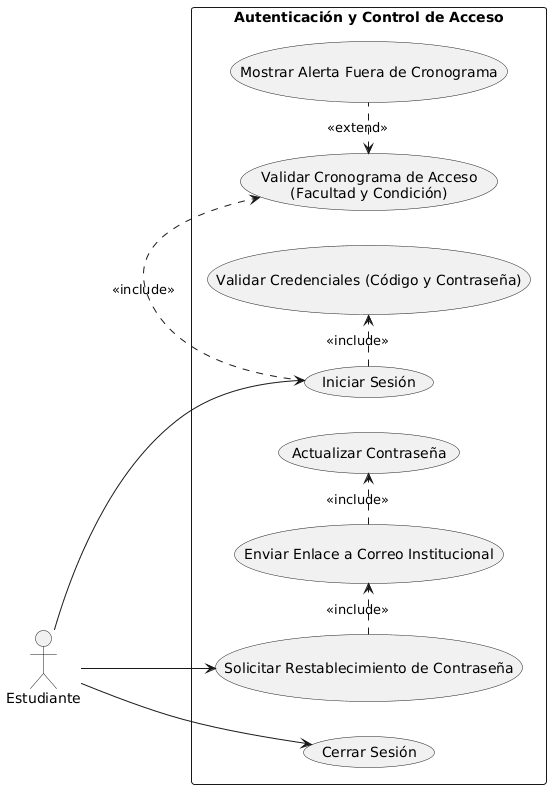
\includegraphics[width=0.82\textwidth]{diagramas/casos-de-uso/imagenes/autenticacion.png}
  \caption{Diagrama de Caso de Uso -- CU-01: Autenticaci\'on y Control de Acceso}
\end{figure}

\begin{longtable}{>{\bfseries\small}p{3.5cm}>{\small}p{11cm}}
  \toprule
  Campo & Descripci\'on \\
  \midrule
  \endfirsthead
  \midrule Campo & Descripci\'on \\ \midrule \endhead
  Id & CU-01 \\
  T\'itulo & Iniciar Sesi\'on y Validar Cronograma (AUTH-LOGIN) \\
  Requerimientos & RF-01, RF-02, RF-03, RF-04 \\
  Prop\'osito & Autenticar la identidad del estudiante y verificar que su acceso corresponda al cronograma asignado. \\
  Actores & Estudiante (iniciador) \\
  Precondiciones & (1) Estudiante registrado y habilitado en BD. (2) Acceso v\'ia navegador a la URL oficial. (3) Cronograma cargado en BD. \\
  Poscondiciones & Sesi\'on autenticada con token JWT. Redirecci\'on condicional: ingresante $\to$ Portafolio, regular $\to$ Cola Virtual. \\
  Flujo Principal & (1) Formulario de inicio de sesi\'on. (2) Ingresa c\'odigo y contrase\~na. (3) El sistema valida credenciales contra BD. (4) Ejecuta \texttt{fn\_validar\_cronograma(id\_escuela, es\_ingresante)}. (5) Redirige seg\'un condici\'on. \\
  Cursos Alternativos & \textbf{4.a} Credenciales incorrectas: mensaje de error, sin sesi\'on. \textbf{5.a} Fuera de cronograma: muestra fecha y hora de turno asignado. \textbf{1.a} Recuperaci\'on de contrase\~na: enlace seguro al correo institucional. \\
  \bottomrule
  \caption{Especificaci\'on CU-01: Iniciar Sesi\'on}
\end{longtable}

\subsection{CU-02: Cargar Documentaci\'on de Portafolio de Admisi\'on}

\begin{figure}[H]
  \centering
  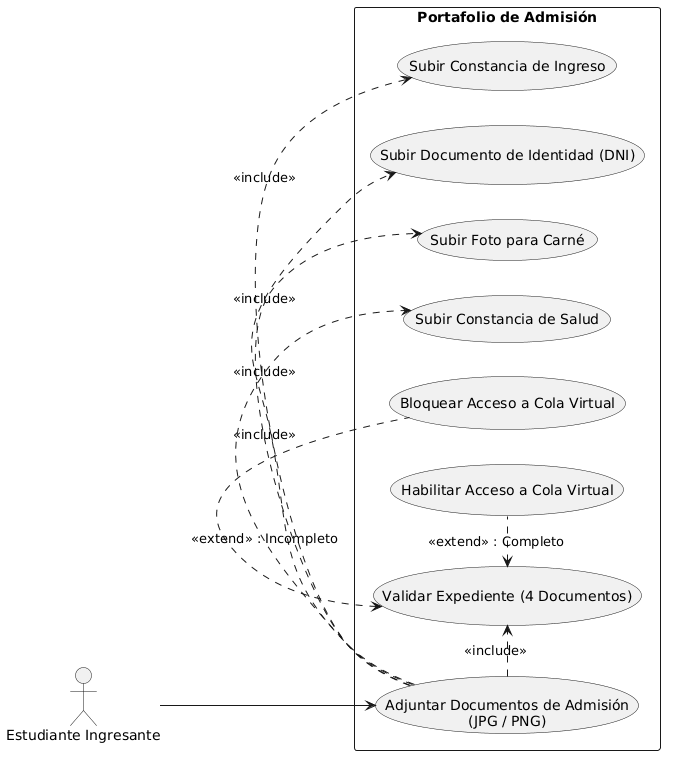
\includegraphics[width=0.82\textwidth]{diagramas/casos-de-uso/imagenes/portafolio.png}
  \caption{Diagrama de Caso de Uso -- CU-02: Portafolio de Admisi\'on (Ingresantes)}
\end{figure}

\begin{longtable}{>{\bfseries\small}p{3.5cm}>{\small}p{11cm}}
  \toprule
  Campo & Descripci\'on \\
  \midrule
  \endfirsthead
  \midrule Campo & Descripci\'on \\ \midrule \endhead
  Id & CU-02 \\
  T\'itulo & Cargar Documentaci\'on de Portafolio de Admisi\'on (PORT-DOCS) \\
  Requerimientos & RF-05, RF-06 \\
  Prop\'osito & Permitir al ingresante adjuntar los 4 documentos obligatorios para habilitar su pase a la matr\'icula. \\
  Actores & Estudiante Ingresante (iniciador) \\
  Precondiciones & (1) Sesi\'on iniciada exitosamente (CU-01). (2) Atributo \texttt{es\_ingresante = TRUE}. \\
  Poscondiciones & Los 4 documentos quedan en \texttt{portafolio\_documento} con estado \texttt{ENTREGADO}. Se habilita el acceso a la Cola Virtual (CU-03). \\
  Flujo Principal & (1) Sistema presenta lista de 4 requisitos. (2) Estudiante selecciona archivo (JPG/PNG, m\'ax. 2 MB). (3) Sistema valida y almacena. (4) Al completar los 4, ejecuta \texttt{fn\_validar\_requisitos\_completos(id\_estudiante)}. (5) Habilita continuaci\'on a CU-03. \\
  Cursos Alternativos & \textbf{5.a} Formato o tama\~no inv\'alido: mensaje de error, carga descartada. \textbf{9.a} Intento de avance incompleto: bloqueo y alerta de documentos pendientes. \\
  \bottomrule
  \caption{Especificaci\'on CU-02: Portafolio de Admisi\'on}
\end{longtable}

\subsection{CU-03: Gestionar Acceso y Turno en Cola Virtual}

\begin{figure}[H]
  \centering
  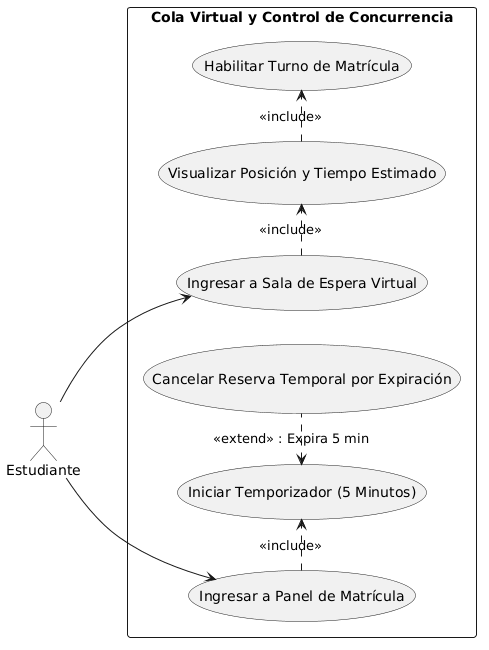
\includegraphics[width=0.82\textwidth]{diagramas/casos-de-uso/imagenes/colavirtual.png}
  \caption{Diagrama de Caso de Uso -- CU-03: Cola Virtual y Control de Concurrencia}
\end{figure}

\begin{longtable}{>{\bfseries\small}p{3.5cm}>{\small}p{11cm}}
  \toprule
  Campo & Descripci\'on \\
  \midrule
  \endfirsthead
  \midrule Campo & Descripci\'on \\ \midrule \endhead
  Id & CU-03 \\
  T\'itulo & Gestionar Acceso y Turno en Cola Virtual (COLA-QUEUE) \\
  Requerimientos & RF-07, RF-08, RF-09 \\
  Prop\'osito & Regular el tr\'afico concurrente mediante una sala de espera virtual con asignaci\'on de turno y temporizador estricto. \\
  Actores & Estudiante (iniciador) \\
  Precondiciones & (1) Autenticaci\'on completada (CU-01). (2) Si ingresante: portafolio completo (CU-02). \\
  Poscondiciones & Sesi\'on activa para selecci\'on de cursos. Temporizador regresivo de 5 minutos iniciado. \\
  Flujo Principal & (1) Estudiante entra a sala de espera. (2) Sistema registra en \texttt{cola\_virtual} con n\'umero correlativo. (3) Muestra turno, posici\'on y tiempo estimado. (4) Polling cada 5 segundos a \texttt{/api/cola/posicion}. (5) Al llegar a posici\'on 1: habilita turno con 300 segundos. (6) Inicia cron\'ometro regresivo. (7) Redirige a CU-04. \\
  Cursos Alternativos & \textbf{6.a} Tiempo expirado: cancela proforma, restituye vacantes, muestra mensaje y redirige a sala de espera. \textbf{Abandono voluntario:} se retira de la cola tras inactividad de sondeo. \\
  \bottomrule
  \caption{Especificaci\'on CU-03: Cola Virtual}
\end{longtable}

\subsection{CU-04: Seleccionar Cursos y Control Concurrente de Vacantes}

\begin{figure}[H]
  \centering
  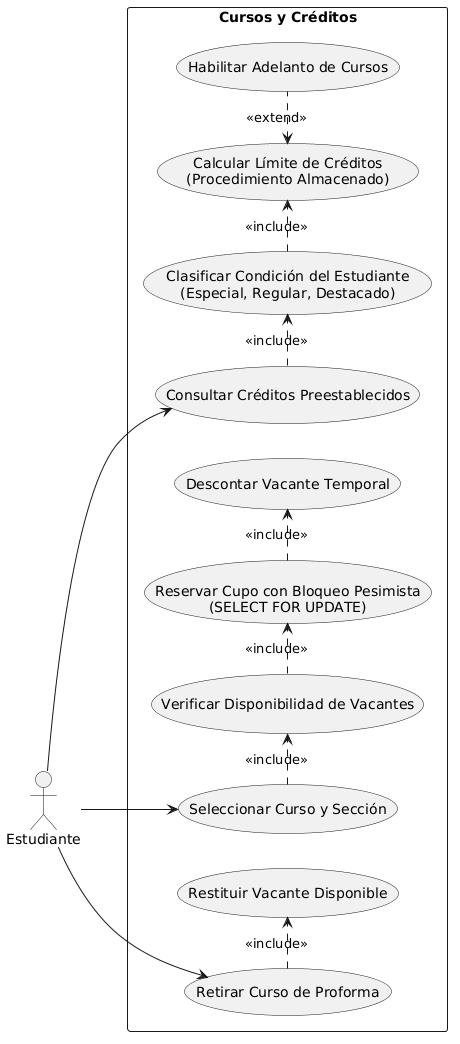
\includegraphics[width=0.82\textwidth]{diagramas/casos-de-uso/imagenes/cursoscreditos.png}
  \caption{Diagrama de Caso de Uso -- CU-04: Datos Acad\'emicos y L\'imite de Cr\'editos}
\end{figure}

\begin{longtable}{>{\bfseries\small}p{3.5cm}>{\small}p{11cm}}
  \toprule
  Campo & Descripci\'on \\
  \midrule
  \endfirsthead
  \midrule Campo & Descripci\'on \\ \midrule \endhead
  Id & CU-04 \\
  T\'itulo & Seleccionar Cursos y Control Concurrente de Vacantes (CURS-SELECC) \\
  Requerimientos & RF-10 a RF-15 \\
  Prop\'osito & Permitir al estudiante seleccionar asignaturas verificando vacantes en tiempo real con bloqueo pesimista. \\
  Actores & Estudiante (iniciador) \\
  Precondiciones & (1) Turno activo con temporizador en curso (CU-03). (2) Matr\'icula no \texttt{CONFIRMADA} en el periodo. \\
  Poscondiciones & Proforma temporal creada/actualizada. Vacante descontada con \texttt{FOR UPDATE}. Acumulador de cr\'editos actualizado. \\
  Flujo Principal & (1) Invoca \texttt{sp\_determinar\_limite\_creditos} para clasificar al alumno. (2) Despliega cat\'alogo de asignaturas. (3) Estudiante elige curso y secci\'on. (4) Sistema ejecuta \texttt{sp\_matricular\_curso} con bloqueo pesimista. (5) Si todo es v\'alido: inserta en \texttt{detalle\_matricula} y descuenta vacante. \\
  Cursos Alternativos & \textbf{6.a} Vacantes agotadas: ROLLBACK y alerta. \textbf{6.b} Exceso de cr\'editos: rechazo con mensaje. \textbf{RF-15} Retiro: remueve de proforma e incrementa vacante. \\
  \bottomrule
  \caption{Especificaci\'on CU-04: Selecci\'on de Cursos}
\end{longtable}

\subsection{CU-05: Visualizar Proforma y Horario Tentativo}

\begin{figure}[H]
  \centering
  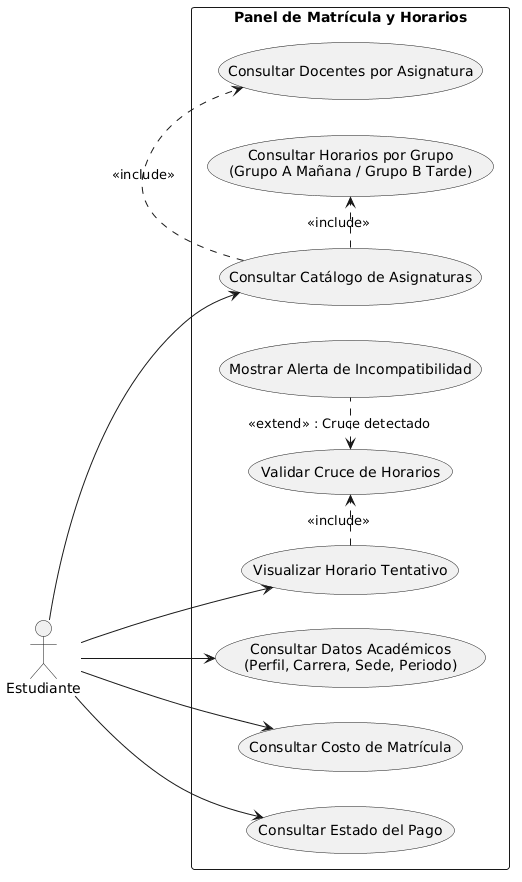
\includegraphics[width=0.82\textwidth]{diagramas/casos-de-uso/imagenes/matricula.png}
  \caption{Diagrama de Caso de Uso -- CU-05: Matr\'icula y Visualizaci\'on de Proforma}
\end{figure}

\begin{longtable}{>{\bfseries\small}p{3.5cm}>{\small}p{11cm}}
  \toprule
  Campo & Descripci\'on \\
  \midrule
  \endfirsthead
  \midrule Campo & Descripci\'on \\ \midrule \endhead
  Id & CU-05 \\
  T\'itulo & Visualizar Proforma y Horario Tentativo (MATR-VPRO) \\
  Requerimientos & RF-10, RF-13, RF-16, RF-17, RF-18 \\
  Prop\'osito & Vista consolidada de la matr\'icula provisional con grilla semanal, detecci\'on de cruces y desglose de costos. \\
  Actores & Estudiante (iniciador) \\
  Precondiciones & Al menos una asignatura agregada a la proforma (CU-04). \\
  Poscondiciones & Grilla horaria renderizada. Si sin cruces: confirmaci\'on habilitada (CU-06). Si con cruces: confirmaci\'on bloqueada. \\
  Flujo Principal & (1) Muestra perfil acad\'emico del estudiante. (2) Renderiza grilla semanal Lunes--S\'abado. (3) Invoca \texttt{fn\_validar\_cruces\_horario(id\_proforma)}. (4) Si sin cruces: muestra asignaturas, cr\'editos, monto y habilita confirmar. \\
  Cursos Alternativos & \textbf{3.a} Cruce detectado: bloques en rojo, alerta de conflicto, bot\'on ``Confirmar'' deshabilitado hasta resolver. \\
  \bottomrule
  \caption{Especificaci\'on CU-05: Visualizaci\'on de Proforma}
\end{longtable}

\subsection{CU-06: Confirmar Matr\'icula y Emitir Ficha Oficial (PDF)}

\begin{figure}[H]
  \centering
  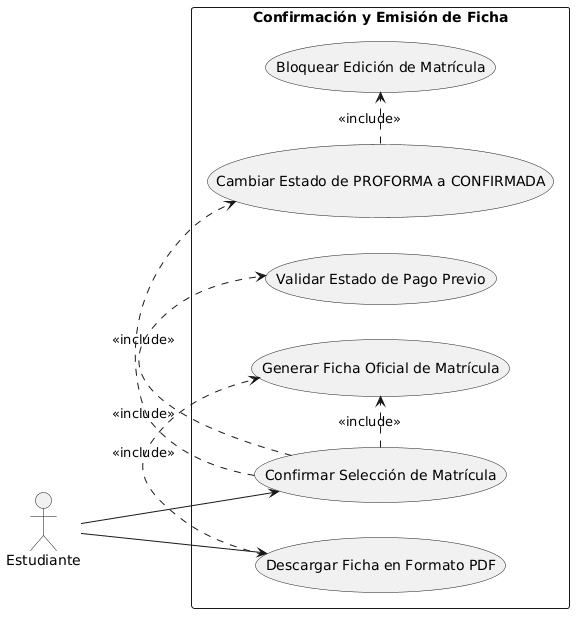
\includegraphics[width=0.82\textwidth]{diagramas/casos-de-uso/imagenes/confirmacion.png}
  \caption{Diagrama de Caso de Uso -- CU-06: Confirmaci\'on y Emisi\'on de Ficha}
\end{figure}

\begin{longtable}{>{\bfseries\small}p{3.5cm}>{\small}p{11cm}}
  \toprule
  Campo & Descripci\'on \\
  \midrule
  \endfirsthead
  \midrule Campo & Descripci\'on \\ \midrule \endhead
  Id & CU-06 \\
  T\'itulo & Confirmar Matr\'icula y Emitir Ficha Oficial (CONF-PDF) \\
  Requerimientos & RF-18, RF-19, RF-20, RF-21 \\
  Prop\'osito & Finalizar la matr\'icula mediante transacci\'on at\'omica y emitir la Ficha Oficial en PDF con c\'odigo de verificaci\'on. \\
  Actores & Estudiante (iniciador) \\
  Precondiciones & (1) Sin cruces de horario (CU-05). (2) Cr\'editos dentro del rango v\'alido. (3) Pago de matr\'icula registrado. (4) Dentro del tiempo l\'imite de 5 minutos (CU-03). \\
  Poscondiciones & Estado cambia de \texttt{PROFORMA} a \texttt{CONFIRMADA}. \texttt{es\_editable = FALSE}. Vacantes consolidadas. Ficha PDF generada con c\'odigo QR. \\
  Flujo Principal & (1) Clic en ``Confirmar Matr\'icula''. (2) Di\'alogo de confirmaci\'on. (3) ``Aceptar y Confirmar''. (4) \texttt{sp\_confirmar\_matricula}: valida pago, actualiza estado, activa inmutabilidad, COMMIT. (5) Muestra confirmaci\'on. (6) Habilita descarga de Ficha PDF. \\
  Cursos Alternativos & \textbf{3.a} Cancelaci\'on en di\'alogo: mantiene proforma editable. \textbf{4.a} Pago pendiente: ROLLBACK y alerta. \textbf{Cr\'editos insuficientes:} bloquea confirmaci\'on con mensaje de m\'inimo requerido. \\
  \bottomrule
  \caption{Especificaci\'on CU-06: Confirmaci\'on de Matr\'icula}
\end{longtable}

\newpage

% ==============================================================================
\section{Diagramas de Secuencia}
% ==============================================================================

Los diagramas de secuencia modelan el flujo de mensajes entre el actor \textbf{Estudiante}, la \textbf{Interfaz Web (React)} y el \textbf{Backend PHP + MySQL} para cada proceso clave del sistema.

\subsection{DS-01: Autenticaci\'on y Validaci\'on de Cronograma}

\begin{figure}[H]
  \centering
  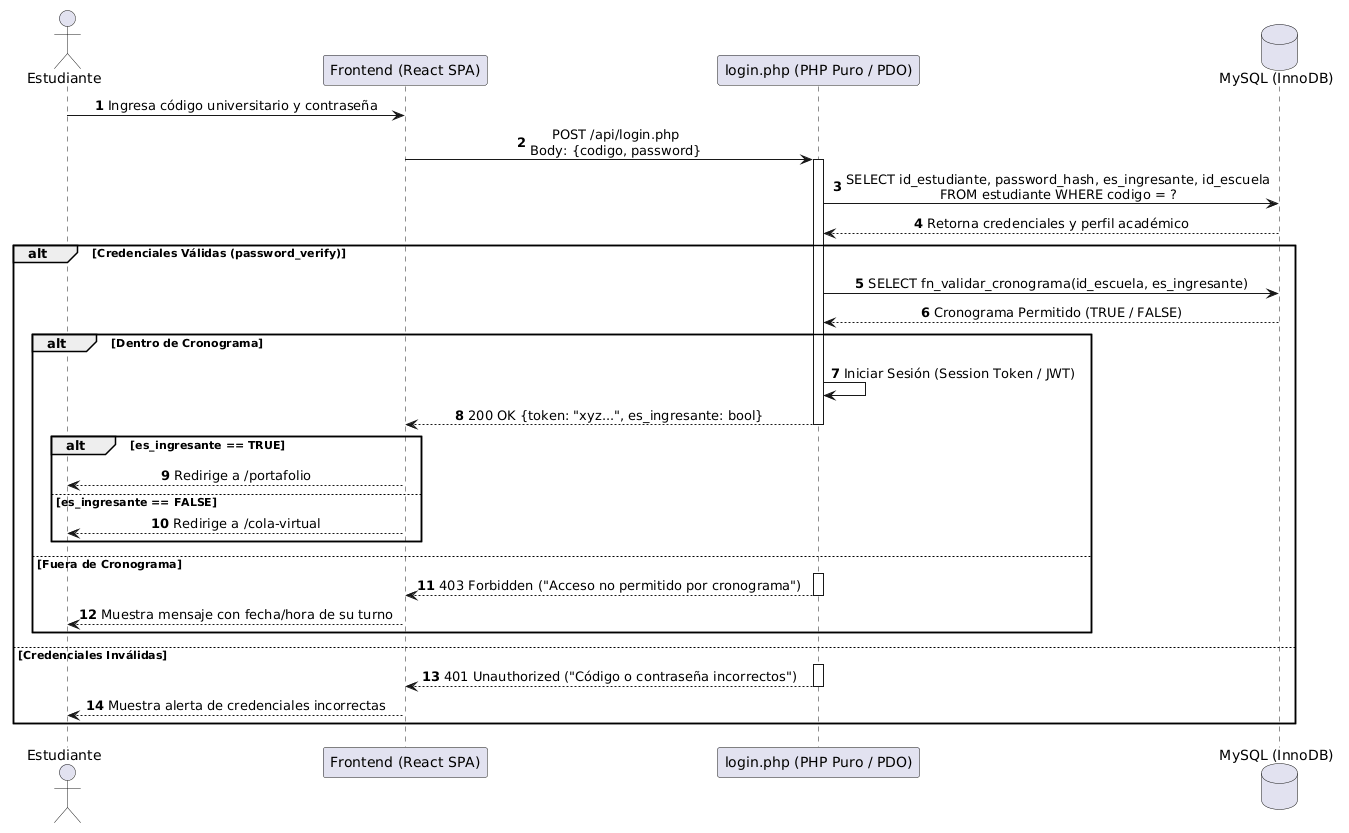
\includegraphics[width=\textwidth]{diagramas/secuencia/imagenes/autenticacion.png}
  \caption{Diagrama de Secuencia -- DS-01: Inicio de Sesi\'on y Validaci\'on de Cronograma}
\end{figure}

El flujo muestra c\'omo el estudiante ingresa credenciales, el backend valida contra la tabla \texttt{estudiante} con hash bcrypt, invoca la funci\'on \texttt{fn\_validar\_cronograma()} para verificar que la hora actual est\'e dentro del rango del cronograma activo y retorna el token JWT con la condici\'on del estudiante para su redirecci\'on condicional.

\subsection{DS-02: Carga de Portafolio de Admisi\'on}

\begin{figure}[H]
  \centering
  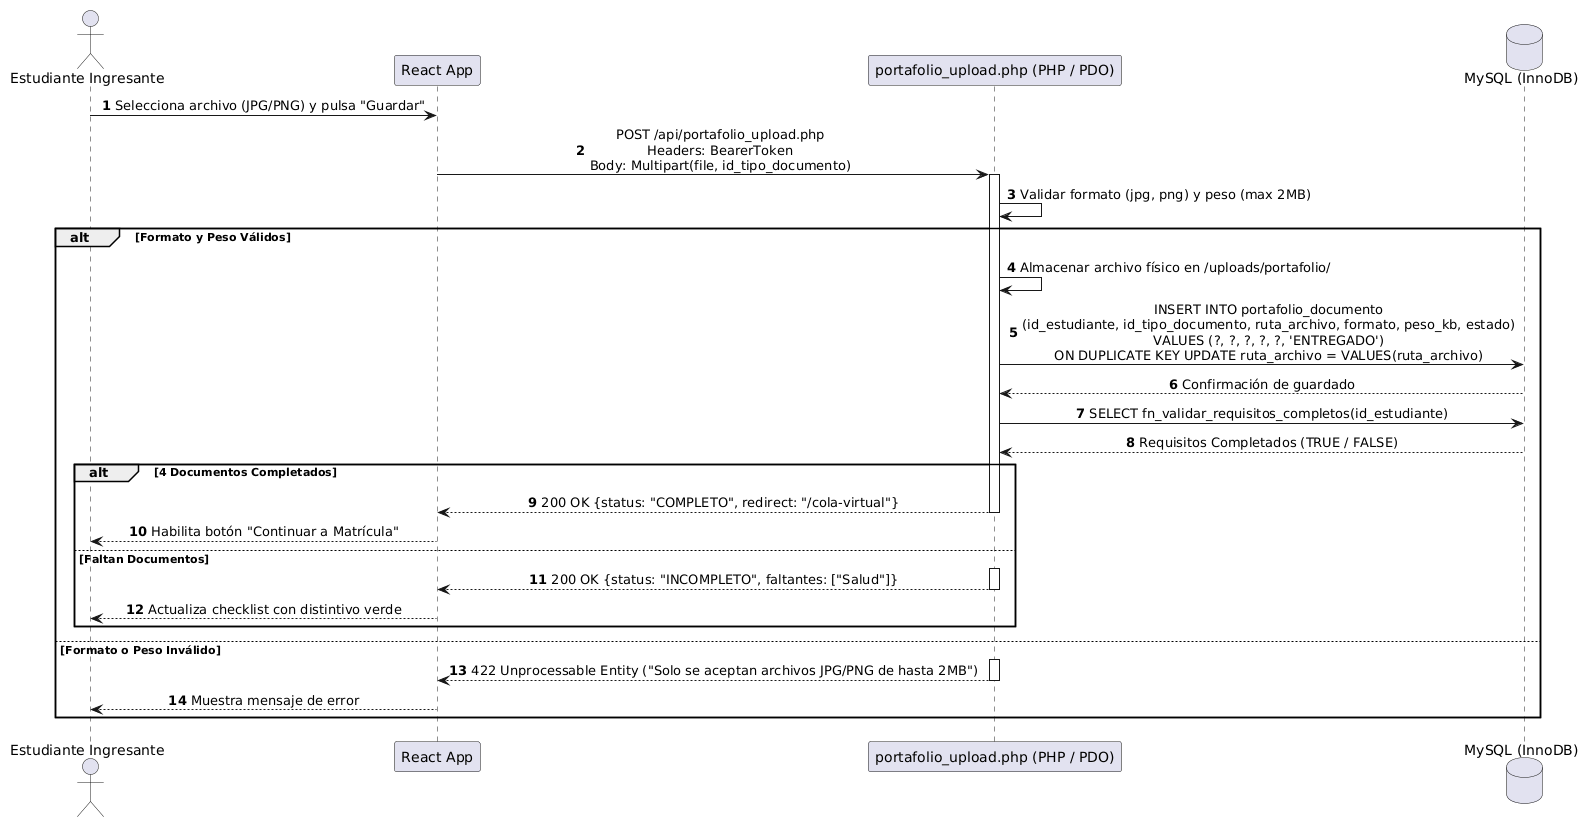
\includegraphics[width=\textwidth]{diagramas/secuencia/imagenes/portafolio.png}
  \caption{Diagrama de Secuencia -- DS-02: Portafolio de Admisi\'on (Ingresantes)}
\end{figure}

El flujo modela la carga de archivos JPG/PNG, la validaci\'on de formato y peso en el servidor, el registro en \texttt{portafolio\_documento} y la invocaci\'on de \texttt{fn\_validar\_requisitos\_completos()} al completar los 4 documentos para habilitar el acceso a la cola.

\subsection{DS-03: Cola Virtual y Temporizador}

\begin{figure}[H]
  \centering
  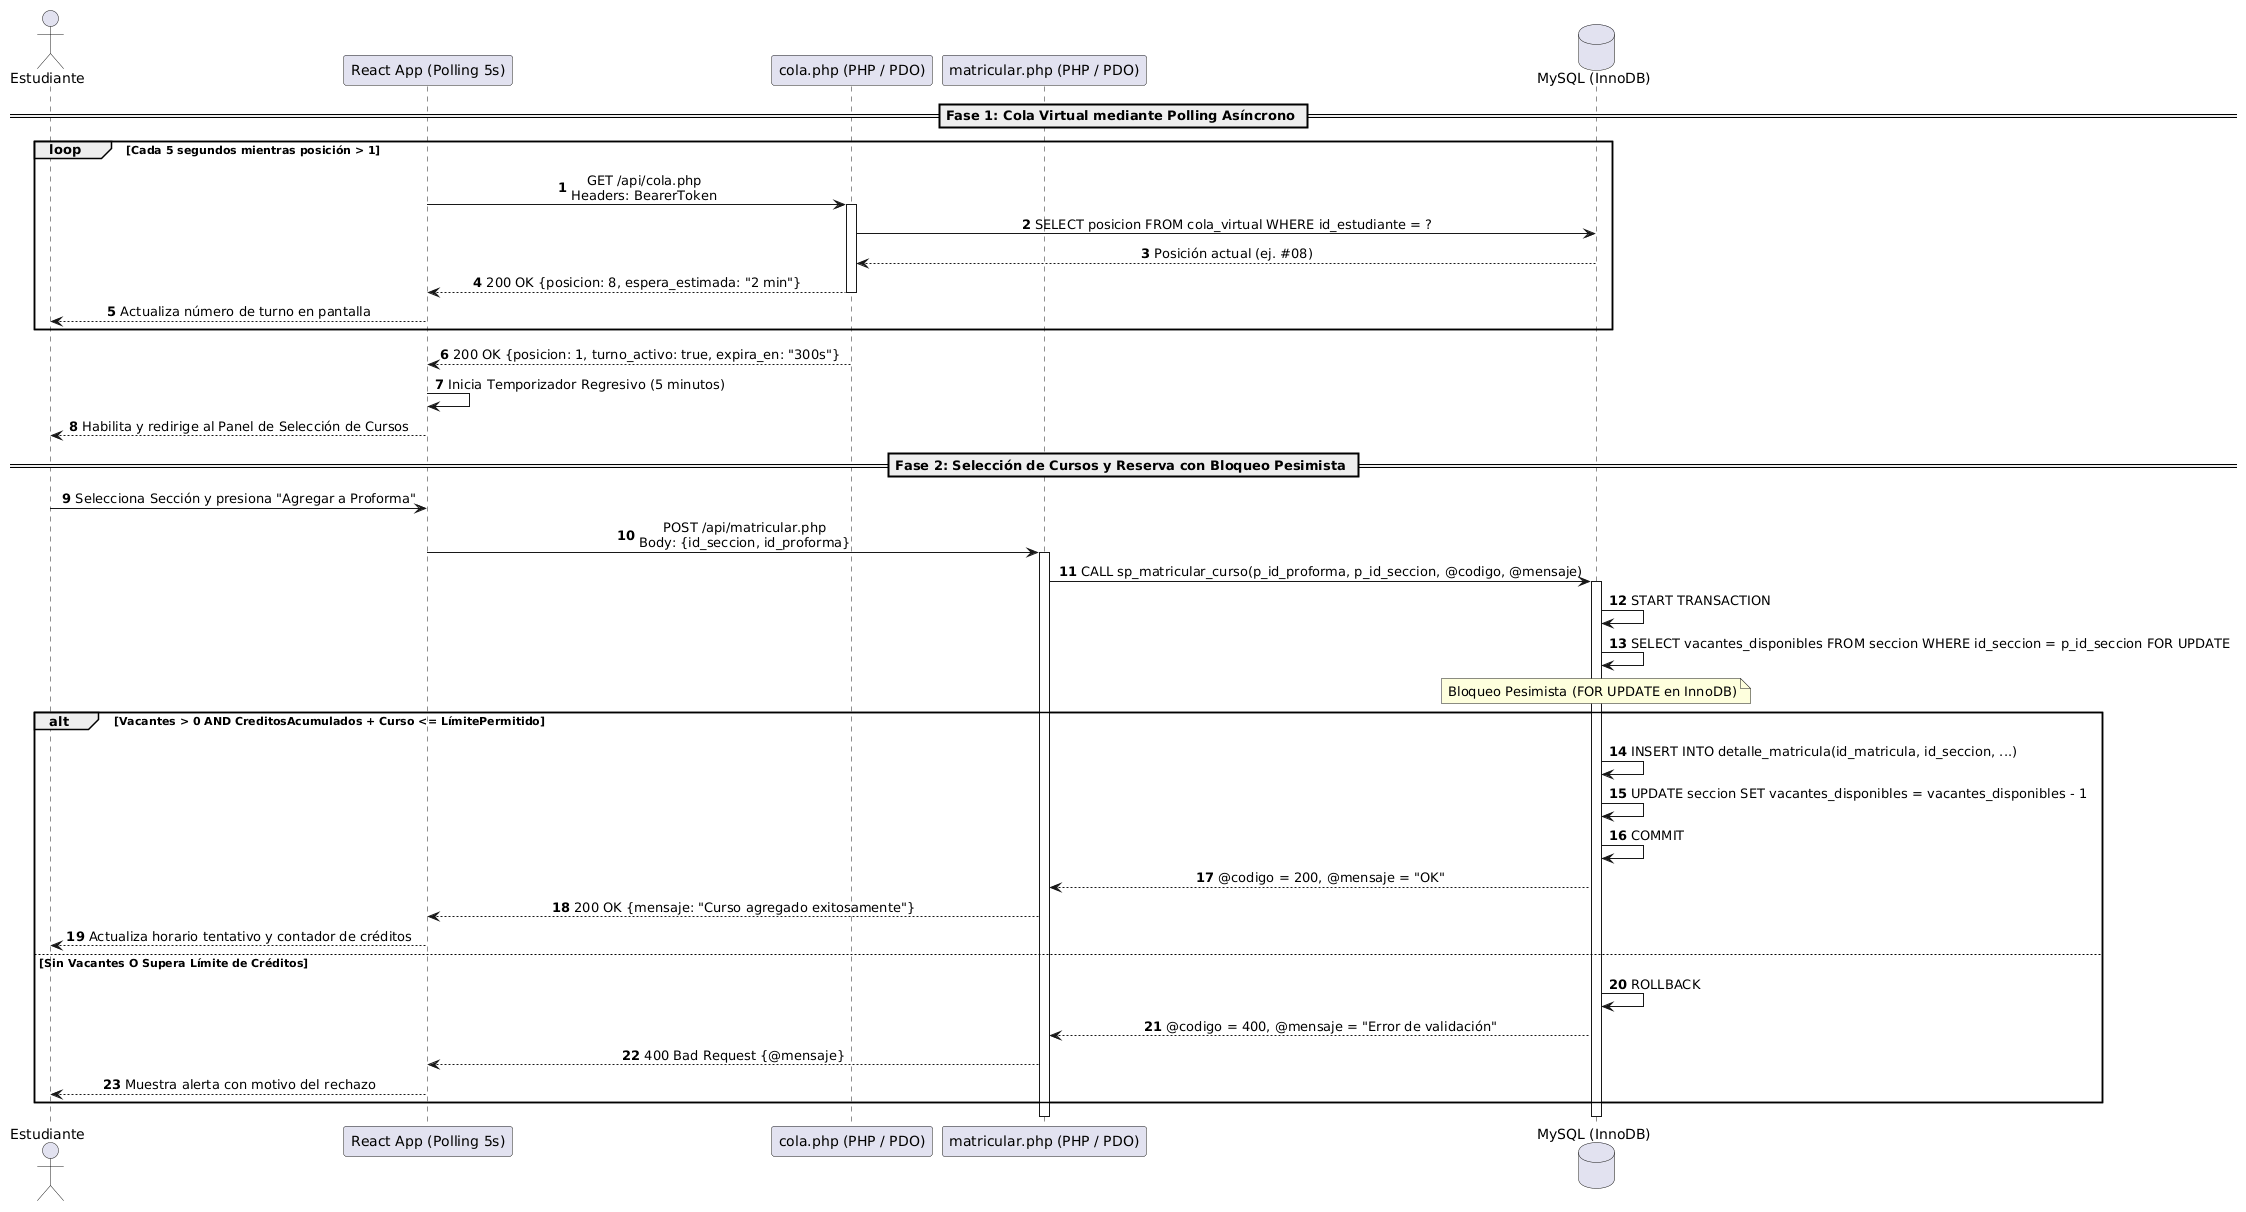
\includegraphics[width=\textwidth]{diagramas/secuencia/imagenes/colavirtual.png}
  \caption{Diagrama de Secuencia -- DS-03: Cola Virtual, Turno y Temporizador de 5 Minutos}
\end{figure}

El diagrama representa el polling peri\'odico (cada 5 segundos) hacia \texttt{/api/cola/posicion}, la activaci\'on del \texttt{TURNO\_HABILITADO} en la tabla \texttt{cola\_virtual}, el inicio del countdown de 300 segundos y el proceso de expiraci\'on que cancela la proforma y restituye vacantes.

\subsection{DS-04: Validaci\'on Transaccional y Confirmaci\'on}

\begin{figure}[H]
  \centering
  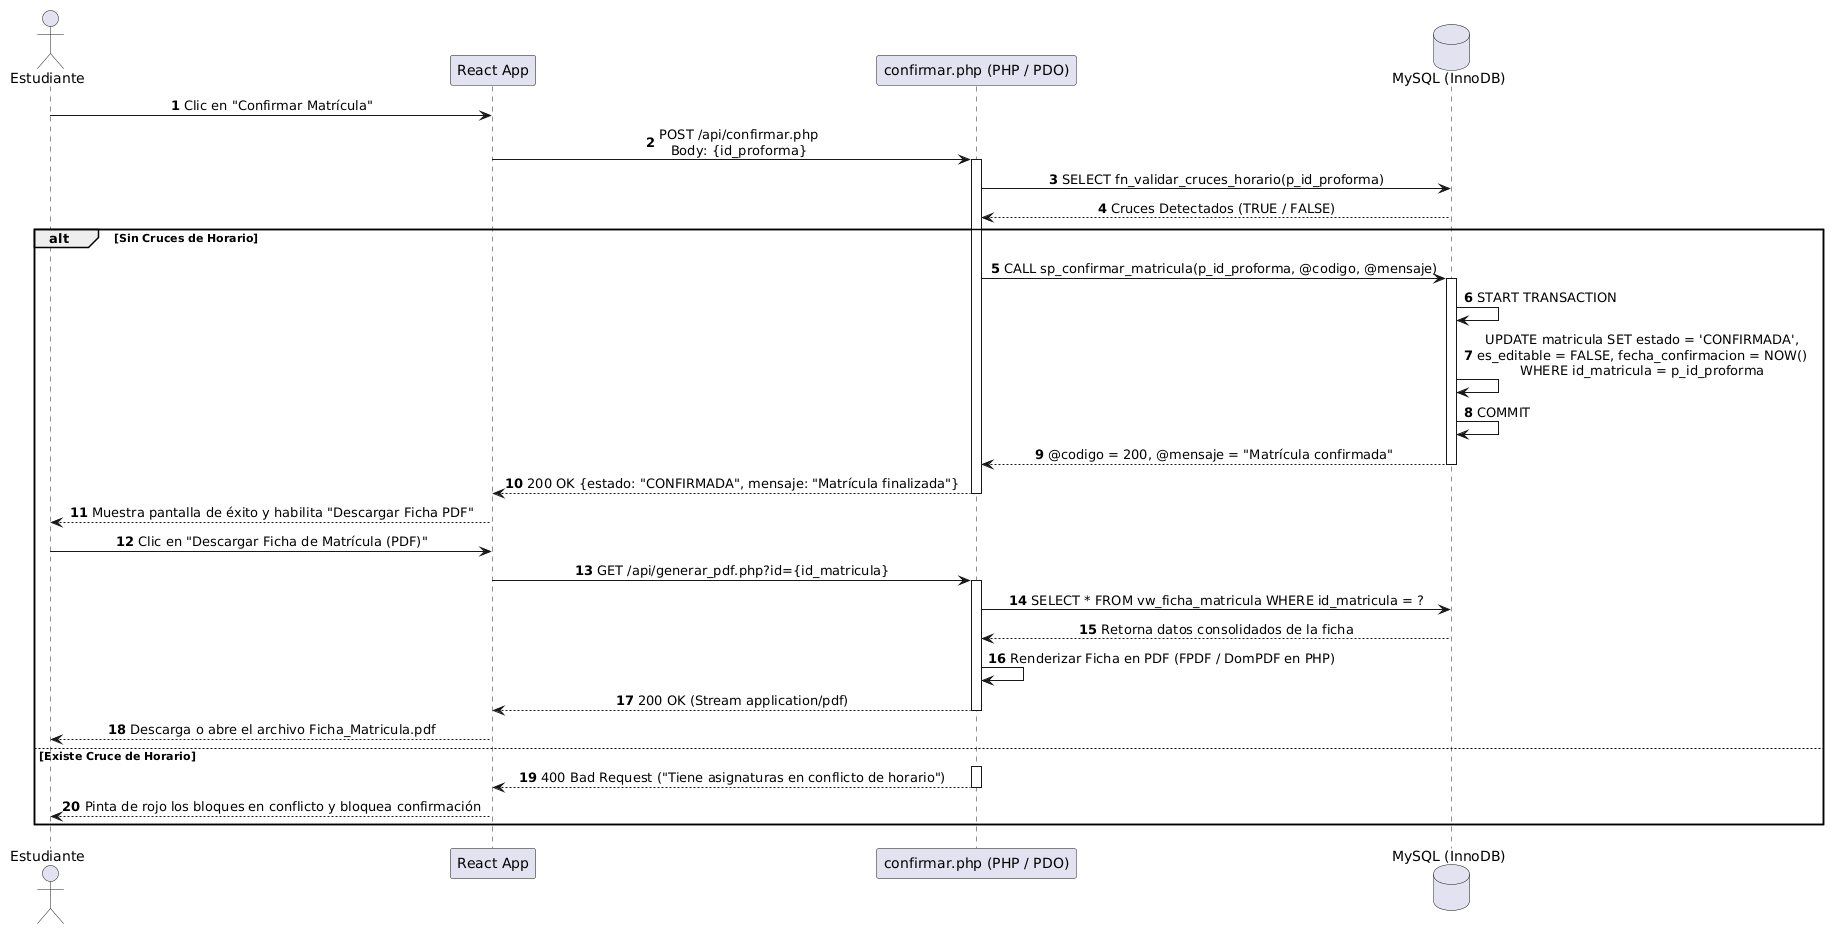
\includegraphics[width=\textwidth]{diagramas/secuencia/imagenes/validacion.png}
  \caption{Diagrama de Secuencia -- DS-04: Validaci\'on de Cr\'editos, Cruces y Confirmaci\'on Transaccional}
\end{figure}

El flujo detalla la secuencia de llamadas al SP \texttt{sp\_matricular\_curso} con bloqueo pesimista \texttt{FOR UPDATE}, la validaci\'on de cruces mediante \texttt{fn\_validar\_cruces\_horario()}, y la transacci\'on at\'omica de \texttt{sp\_confirmar\_matricula} que transiciona el estado de \texttt{PROFORMA} a \texttt{CONFIRMADA}.

\newpage

% ==============================================================================
\section{Mockups de Interfaz (Figma)}
% ==============================================================================

Los prototipos de pantalla del sistema fueron dise\~nados en \textbf{Figma} como parte del proceso de dise\~no centrado en el usuario, estableciendo la gu\'ia visual, la arquitectura de informaci\'on y la experiencia de flujo antes del desarrollo. A continuaci\'on se presentan los mockups de las pantallas principales implementadas:

\subsection{Pantalla: Inicio de Sesi\'on}

\begin{figure}[H]
  \centering
  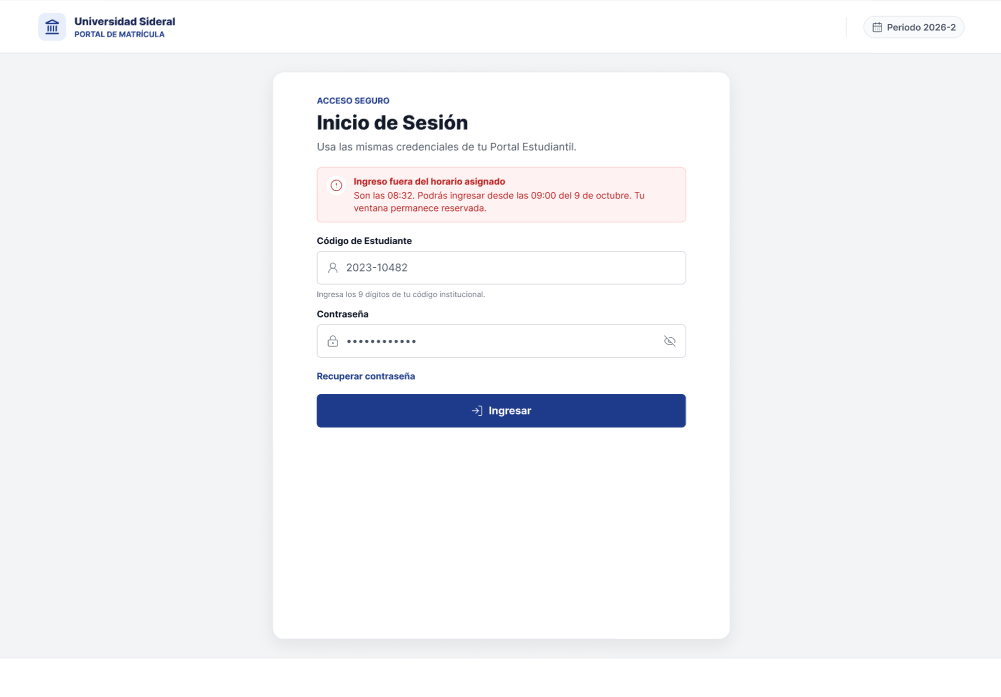
\includegraphics[width=0.90\textwidth]{mockups/inicio_sesion.png}
  \caption{Mockup -- Pantalla de Inicio de Sesi\'on (Figma)}
\end{figure}

Formulario de autenticaci\'on con campos de c\'odigo universitario y contrase\~na. Incluye el enlace de recuperaci\'on de contrase\~na y la identidad visual de la UNJBG con fondo de gradiente oscuro.

\subsection{Pantalla: Portafolio de Admisi\'on}

\begin{figure}[H]
  \centering
  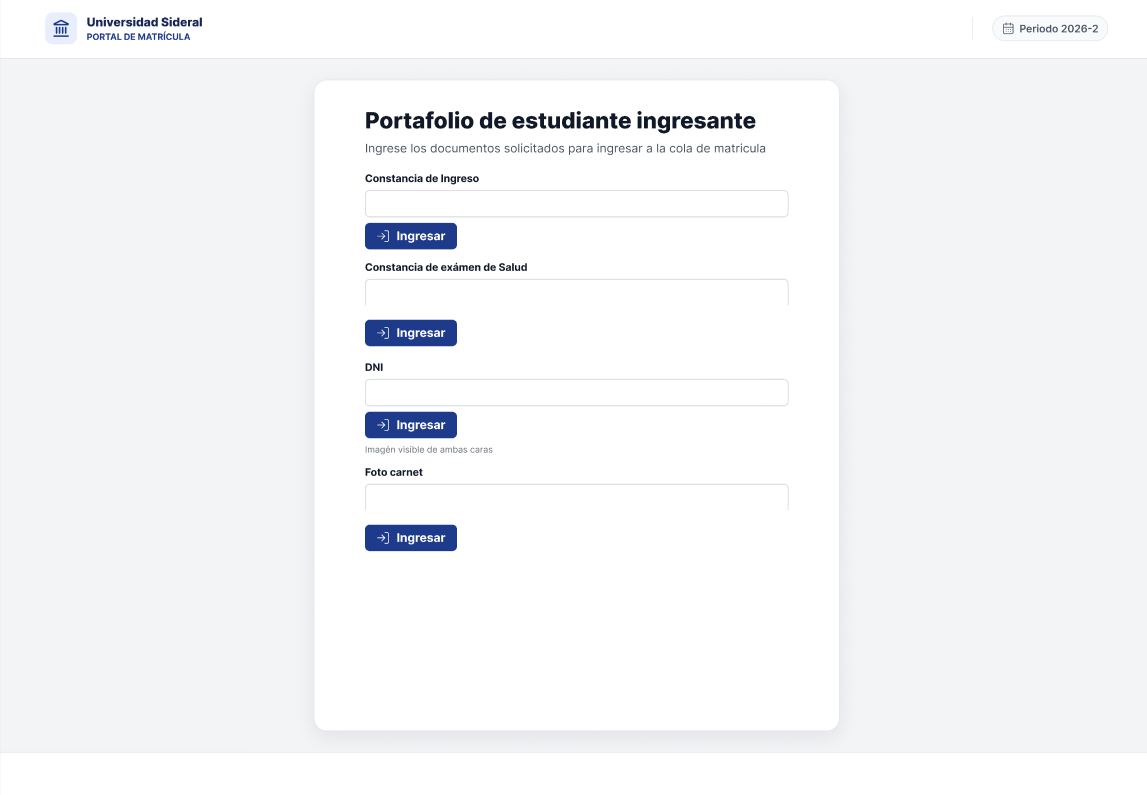
\includegraphics[width=0.90\textwidth]{mockups/portafolio.png}
  \caption{Mockup -- Pantalla de Portafolio de Admisi\'on (Figma)}
\end{figure}

Panel exclusivo para estudiantes ingresantes que muestra la lista de 4 requisitos de admisi\'on con indicadores visuales de estado (Pendiente / Entregado), botones de carga individuales y un indicador de progreso general.

\subsection{Pantalla: Cola Virtual}

\begin{figure}[H]
  \centering
  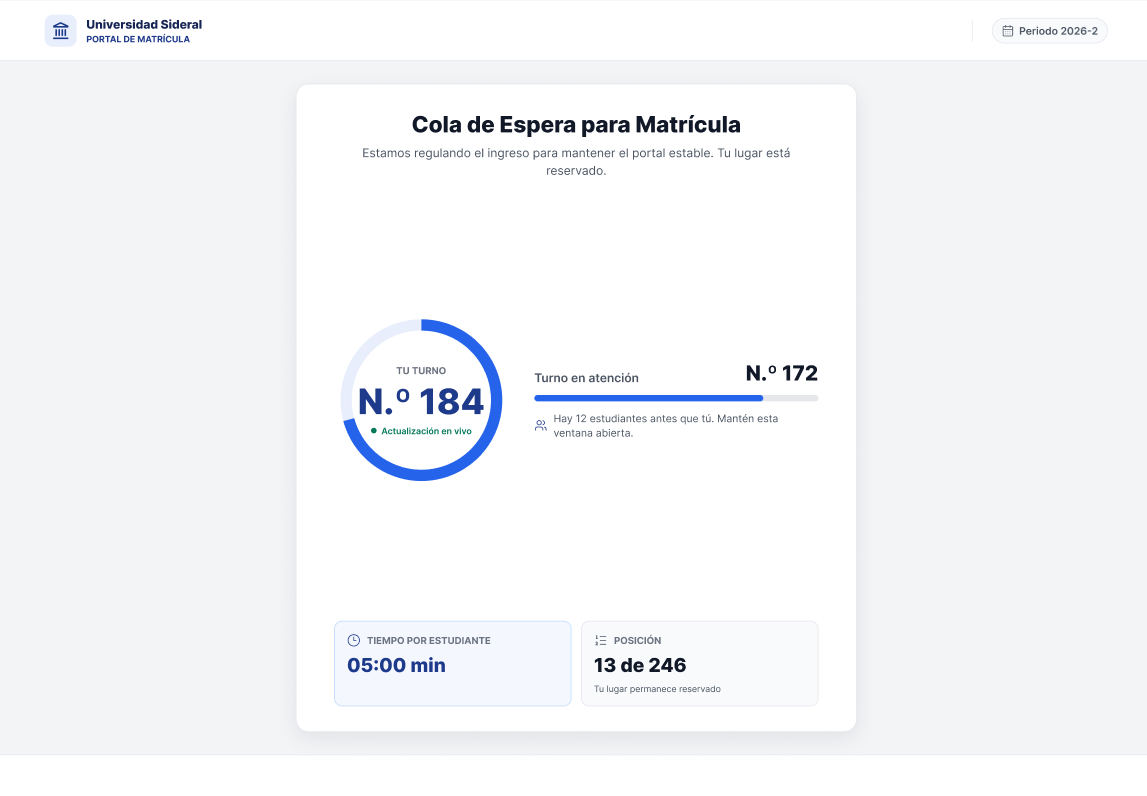
\includegraphics[width=0.90\textwidth]{mockups/cola.png}
  \caption{Mockup -- Pantalla de Cola Virtual y Sala de Espera (Figma)}
\end{figure}

Sala de espera virtual que muestra el n\'umero de turno del estudiante, su posici\'on en la fila, el tiempo estimado de espera y el temporizador regresivo de 5 minutos cuando el turno se activa.

\subsection{Pantalla: Panel de Matr\'icula}

\begin{figure}[H]
  \centering
  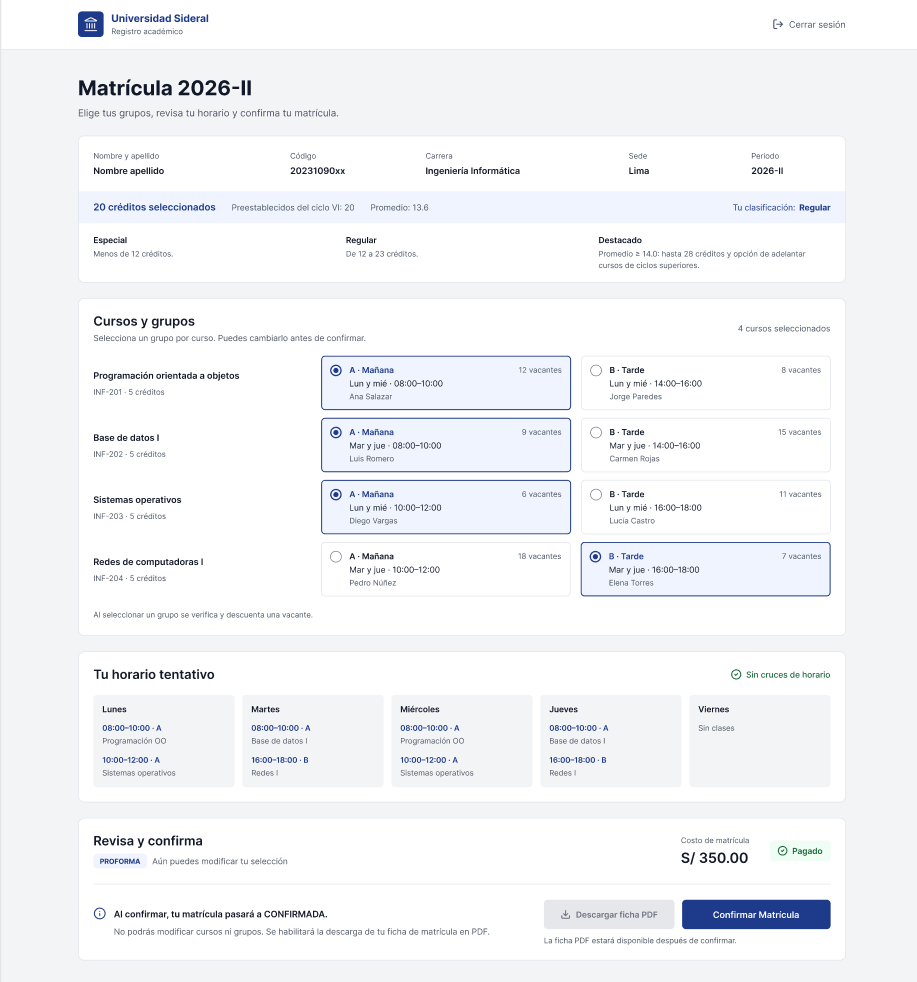
\includegraphics[width=0.90\textwidth]{mockups/matricula.png}
  \caption{Mockup -- Panel de Selecci\'on de Cursos y Horario Tentativo (Figma)}
\end{figure}

Panel principal de matr\'icula con el cat\'alogo de asignaturas disponibles (con grupos, horarios, docentes y vacantes en tiempo real), la grilla semanal tentativa y la barra inferior con total de cr\'editos, monto de pago y bot\'on de confirmaci\'on.

\newpage

% ==============================================================================
\section{Modelo Relacional y Diccionario de Datos}
% ==============================================================================

\subsection{Diagrama del Modelo Relacional}

El modelo relacional ha sido dise\~nado en \textbf{Tercera Forma Normal (3FN)} con \textbf{18 tablas} normalizadas, motor \textbf{InnoDB} para soporte de transacciones ACID y bloqueos a nivel de fila.

\begin{figure}[H]
  \centering
  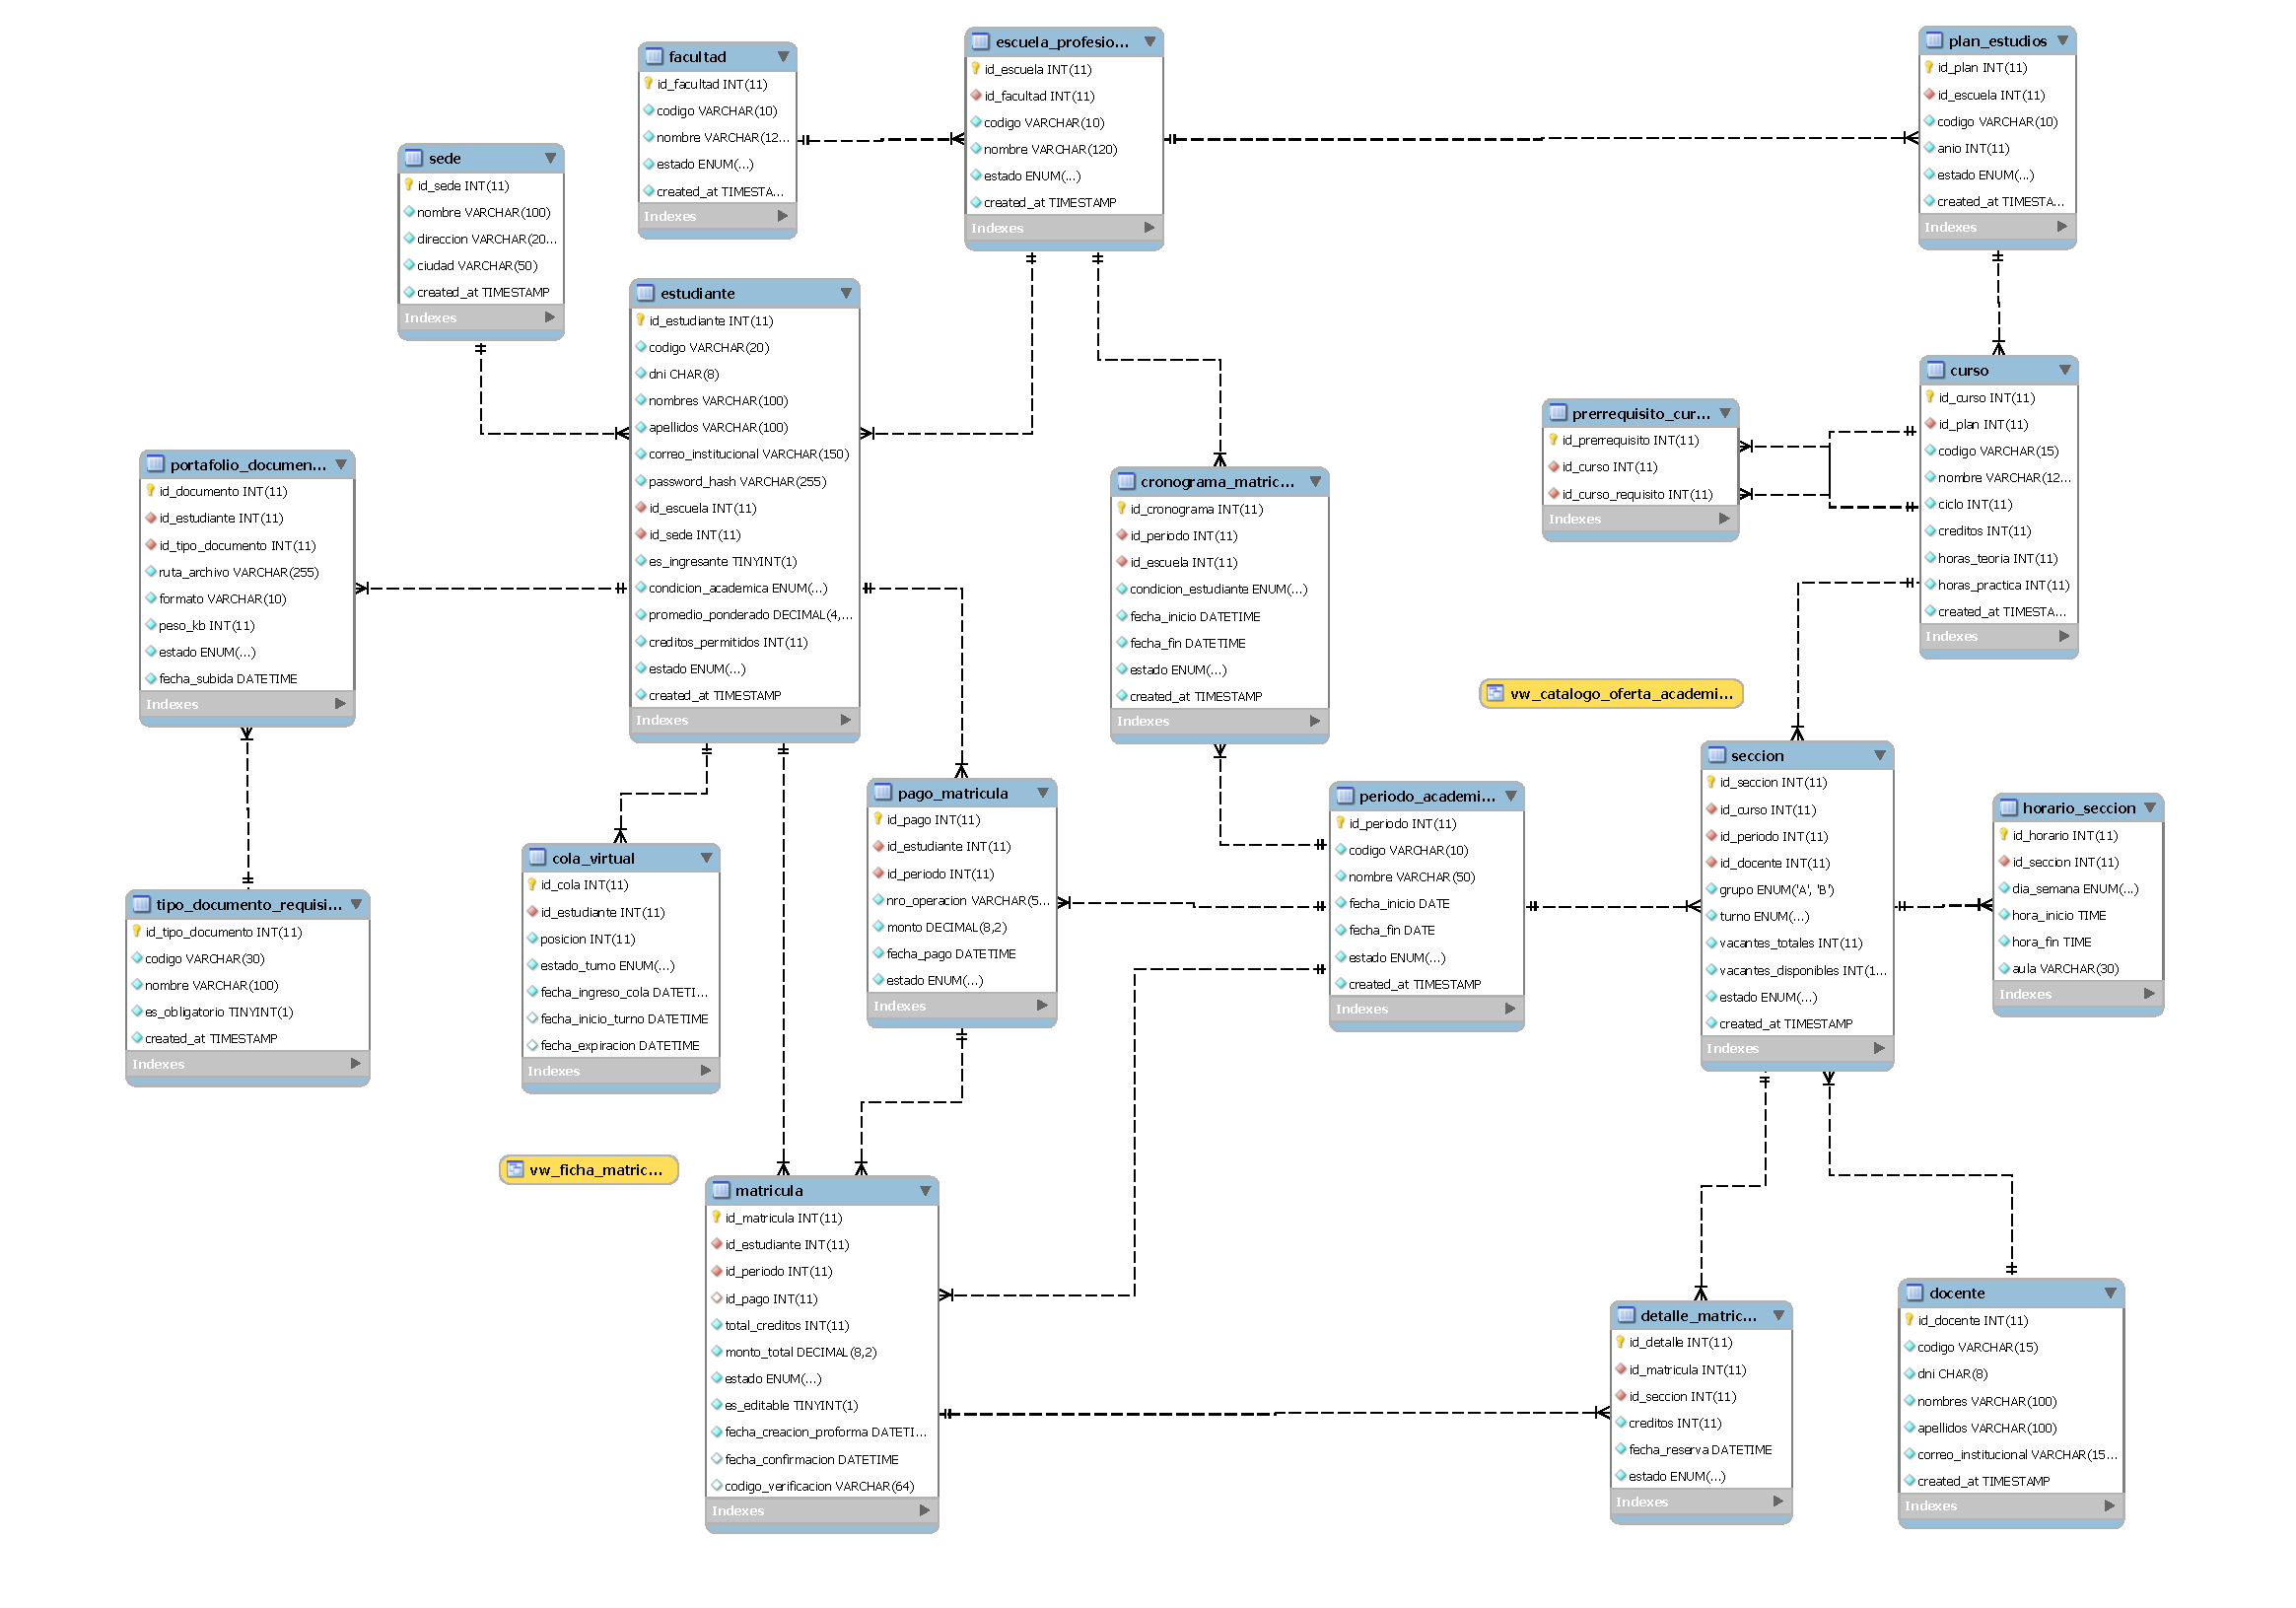
\includegraphics[width=\textwidth]{modelo_relacional.pdf}
  \caption{Modelo Relacional -- Sistema Web de Matr\'icula UNJBG (3FN)}
\end{figure}

\subsection{Descripci\'on de Tablas y Campos Clave}

\subsubsection{\'Area 1: Estructura Acad\'emica e Institucional}

\textbf{Tabla \texttt{facultad}:} Representa las unidades acad\'emicas mayores (ej. Facultad de Ingenier\'ia). Campos clave: \texttt{id\_facultad} (PK), \texttt{codigo} (c\'odigo \'unico, ej. ``FAING''), \texttt{nombre}, \texttt{estado} (ACTIVO/INACTIVO).

\textbf{Tabla \texttt{escuela\_profesional}:} Especialidades adscritas a cada facultad. El campo \texttt{id\_facultad} (FK) establece la relaci\'on 1:N. Contiene el \texttt{codigo} de carrera (ej. ``ESIS'') y su estado.

\textbf{Tabla \texttt{sede}:} Campus f\'isicos de la universidad (ej. Sede Central Capanique, Sede Tarata). Referenciada por \texttt{estudiante}.

\textbf{Tabla \texttt{periodo\_academico}:} Ciclos semestrales lectivos (ej. ``2026-II''). El campo \texttt{estado} controla si el periodo est\'a en \texttt{PLANIFICACION}, \texttt{ACTIVO} o \texttt{CERRADO}. Solo periodos \texttt{ACTIVO} admiten operaciones de matr\'icula.

\subsubsection{\'Area 2: Estudiantes y Control de Acceso}

\textbf{Tabla \texttt{estudiante}:} Entidad central del sistema. Almacena datos biogr\'aficos, credenciales (\texttt{password\_hash} con bcrypt) y los tres campos determinantes para la matr\'icula:
\begin{itemize}
  \item \texttt{es\_ingresante} (BOOLEAN): define el flujo de acceso (portafolio o cola directa).
  \item \texttt{condicion\_academica} (ESPECIAL/REGULAR/DESTACADO): determina el tope de cr\'editos.
  \item \texttt{promedio\_ponderado}: base para clasificar como Destacado ($\geq 14.0$).
\end{itemize}

\textbf{Tabla \texttt{cronograma\_matricula}:} Regula la ventana de tiempo (fecha/hora inicio y fin) en que cada escuela y condici\'on de estudiante puede ingresar. La funci\'on \texttt{fn\_validar\_cronograma()} consulta esta tabla para permitir o bloquear el acceso.

\subsubsection{\'Area 3: Portafolio de Requisitos de Admisi\'on}

\textbf{Tabla \texttt{tipo\_documento\_requisito}:} Cat\'alogo fijo de los 4 documentos obligatorios de admisi\'on: \texttt{CONSTANCIA\_INGRESO}, \texttt{DNI}, \texttt{FOTO\_CARNE}, \texttt{EXAMEN\_SALUD}.

\textbf{Tabla \texttt{portafolio\_documento}:} Almacena metadatos de las im\'agenes adjuntas: \texttt{ruta\_archivo} en el servidor, \texttt{formato} (JPG/PNG), \texttt{peso\_kb} (m\'ax. 2048 KB) y \texttt{estado} (PENDIENTE/ENTREGADO/VALIDADO).

\subsubsection{\'Area 4: Cola Virtual y Concurrencia}

\textbf{Tabla \texttt{cola\_virtual}:} Gestiona la sala de espera. Los campos cr\'iticos son:
\begin{itemize}
  \item \texttt{posicion}: n\'umero de orden correlativo en la fila.
  \item \texttt{estado\_turno}: ciclo de vida (EN\_ESPERA $\to$ TURNO\_HABILITADO $\to$ FINALIZADO/EXPIRADO).
  \item \texttt{fecha\_expiracion}: timestamp exacto de los 5 minutos de acceso asignados.
\end{itemize}
La restricci\'on \texttt{UNIQUE(id\_estudiante)} garantiza que un alumno solo tenga un registro activo.

\subsubsection{\'Area 5: Plan de Estudios, Oferta Acad\'emica y Horarios}

\textbf{Tabla \texttt{plan\_estudios}:} Versi\'on curricular de cada carrera. Referenciada por \texttt{curso}.

\textbf{Tabla \texttt{curso}:} Materias del plan de estudios con \texttt{ciclo}, \texttt{creditos}, \texttt{horas\_teoria} y \texttt{horas\_practica}. El \texttt{codigo} es \'unico (ej. ``IS-501'').

\textbf{Tabla \texttt{prerrequisito\_curso}:} Relaci\'on reflexiva sobre \texttt{curso}: modela que un curso exige haber aprobado uno o m\'as cursos previos. Usa dos FK hacia \texttt{curso}: \texttt{id\_curso} (destino) e \texttt{id\_curso\_requisito} (prerrequisito).

\textbf{Tabla \texttt{docente}:} Registro del personal docente con c\'odigo institucional, DNI y correo.

\textbf{Tabla \texttt{seccion}:} \textbf{Tabla cr\'itica para el control de concurrencia.} Cada fila representa una oferta concreta de un curso para un periodo y un docente. Campos fundamentales:
\begin{itemize}
  \item \texttt{grupo} (A/B) y \texttt{turno} (MA\~NANA/TARDE): identifican la secci\'on.
  \item \texttt{vacantes\_disponibles}: campo sobre el que opera el bloqueo pesimista \texttt{SELECT ... FOR UPDATE}, garantizando que nunca se exceda la capacidad f\'isica.
\end{itemize}

\textbf{Tabla \texttt{horario\_seccion}:} Distribuci\'on semanal de bloques de clase: \texttt{dia\_semana} (LUNES...S\'ABADO), \texttt{hora\_inicio}, \texttt{hora\_fin} y \texttt{aula}. Empleada por \texttt{fn\_validar\_cruces\_horario()} para detectar solapamientos.

\subsubsection{\'Area 6: Proforma, Pagos y Confirmaci\'on}

\textbf{Tabla \texttt{pago\_matricula}:} Registra el comprobante de pago: \texttt{nro\_operacion} (\'unico, voucher bancario), \texttt{monto}, \texttt{fecha\_pago} y \texttt{estado} (PENDIENTE/PAGADO). Un pago \texttt{PAGADO} es condici\'on obligatoria para confirmar la matr\'icula.

\textbf{Tabla \texttt{matricula}:} \textbf{Entidad central del proceso transaccional.} Administra el ciclo de vida mediante:
\begin{itemize}
  \item \texttt{estado} (PROFORMA $\to$ CONFIRMADA): transici\'on controlada exclusivamente por \texttt{sp\_confirmar\_matricula}.
  \item \texttt{es\_editable} (BOOLEAN): en \texttt{TRUE} permite agregar/retirar cursos; al confirmar pasa a \texttt{FALSE} de forma permanente.
  \item \texttt{codigo\_verificacion}: hash SHA-256 \'unico para el QR de la ficha PDF.
  \item Restricci\'on \texttt{UNIQUE(id\_estudiante, id\_periodo)}: garantiza una sola matr\'icula por alumno por semestre.
\end{itemize}

\textbf{Tabla \texttt{detalle\_matricula}:} Registra cada secci\'on agregada por el alumno durante la proforma. El campo \texttt{estado} (RESERVADO\_TEMPORAL $\to$ CONFIRMADO) refleja si la reserva de cupo es provisional o definitiva.

\newpage

% ==============================================================================
\section{Procedimientos Almacenados, Funciones y Vistas}
% ==============================================================================

Esta secci\'on describe los objetos de base de datos programables implementados en MySQL, explicando su prop\'osito, los par\'ametros que reciben y la raz\'on t\'ecnica por la que fueron creados en la capa de base de datos.

\subsection{Procedimientos Almacenados (Stored Procedures)}

\subsubsection{SP-01: \texttt{sp\_determinar\_limite\_creditos}}

\textbf{Prop\'osito:} Clasifica la condici\'on acad\'emica del estudiante y determina su bolsa de cr\'editos permitida para el periodo vigente.

\textbf{Justificaci\'on:} La regla de negocio depende de datos estrictamente relacionales (promedio, historial). Calcularla en MySQL garantiza consistencia incluso si m\'ultiples clientes consumen la BD simult\'aneamente.

\begin{lstlisting}[language=SQL, caption={Interfaz de sp\_determinar\_limite\_creditos}]
CALL sp_determinar_limite_creditos(
    IN  p_id_estudiante INT,
    OUT p_condicion     VARCHAR(20),  -- ESPECIAL | REGULAR | DESTACADO
    OUT p_min_creditos  INT,          -- Minimo requerido
    OUT p_max_creditos  INT           -- Maximo permitido
);
-- Logica:
-- IF promedio >= 14.0  --> DESTACADO, min=0,  max=28
-- IF promedio >= 11.0  --> REGULAR,   min=12, max=23
-- ELSE                 --> ESPECIAL,  min=0,  max=11
\end{lstlisting}

\subsubsection{SP-02: \texttt{sp\_matricular\_curso}}

\textbf{Prop\'osito:} Reserva una vacante en una secci\'on para la proforma de un estudiante, aplicando \textbf{bloqueo pesimista} para garantizar que dos estudiantes concurrentes no tomen el \'ultimo cupo disponible.

\textbf{Justificaci\'on:} Es el punto m\'as cr\'itico de concurrencia del sistema. El \texttt{SELECT ... FOR UPDATE} a nivel de motor InnoDB bloquea la fila de la secci\'on durante la transacci\'on, lo cual es imposible de garantizar desde c\'odigo PHP con la misma atomicidad.

\begin{lstlisting}[language=SQL, caption={Logica central de sp\_matricular\_curso}]
START TRANSACTION;
  -- BLOQUEO PESIMISTA sobre la fila de la seccion
  SELECT vacantes_disponibles INTO v_vacantes
  FROM seccion WHERE id_seccion = p_id_seccion FOR UPDATE;

  IF v_vacantes <= 0 THEN
    SIGNAL SQLSTATE '45000'
      SET MESSAGE_TEXT = 'Vacantes agotadas en la seccion seleccionada';
    ROLLBACK;
  ELSE
    UPDATE seccion
      SET vacantes_disponibles = vacantes_disponibles - 1
    WHERE id_seccion = p_id_seccion;

    INSERT INTO detalle_matricula
      (id_matricula, id_seccion, creditos, fecha_reserva, estado)
    VALUES
      (p_id_proforma, p_id_seccion, v_creditos, NOW(),
       'RESERVADO_TEMPORAL');

    UPDATE matricula
      SET total_creditos = total_creditos + v_creditos
    WHERE id_matricula = p_id_proforma;

    COMMIT;
  END IF;
\end{lstlisting}

\subsubsection{SP-03: \texttt{sp\_confirmar\_matricula}}

\textbf{Prop\'osito:} Ejecuta la transacci\'on at\'omica que consolida definitivamente la matr\'icula, transitando el estado de \texttt{PROFORMA} a \texttt{CONFIRMADA} y bloqueando toda edici\'on futura.

\textbf{Justificaci\'on:} Una confirmaci\'on involucra m\'ultiples escrituras que deben ser at\'omicas. Si cualquiera falla, el \texttt{ROLLBACK} garantiza que la BD quede en estado consistente.

\begin{lstlisting}[language=SQL, caption={Logica central de sp\_confirmar\_matricula}]
START TRANSACTION;
  -- Valida creditos minimos segun condicion academica
  IF v_total_creditos < v_min_creditos THEN
    ROLLBACK;
    LEAVE proc_body;
  END IF;

  -- Genera hash de verificacion SHA-256 unico
  SET v_hash = SHA2(CONCAT(p_id_proforma, NOW(), RAND()), 256);

  -- Transicion de estado: PROFORMA --> CONFIRMADA
  UPDATE matricula
  SET estado = 'CONFIRMADA',
      es_editable = FALSE,
      fecha_confirmacion = NOW(),
      codigo_verificacion = v_hash
  WHERE id_matricula = p_id_proforma;

  -- Consolida los detalles de la proforma
  UPDATE detalle_matricula
    SET estado = 'CONFIRMADO'
  WHERE id_matricula = p_id_proforma;

  -- Marca el turno de la cola como finalizado
  UPDATE cola_virtual
    SET estado_turno = 'FINALIZADO'
  WHERE id_estudiante = v_id_estudiante;

COMMIT;
\end{lstlisting}

\subsection{Funciones Deterministas (Functions)}

\subsubsection{FN-01: \texttt{fn\_validar\_cronograma}}

\textbf{Prop\'osito:} Verifica si la fecha y hora actual del servidor se encuentran dentro del rango de acceso permitido para una escuela y condici\'on de estudiante.

\textbf{Justificaci\'on:} Centraliza la l\'ogica de control de acceso temporal en un \'unico punto, evitando que la validaci\'on sea replicada en m\'ultiples endpoints PHP donde podr\'ia ser manipulada.

\begin{lstlisting}[language=SQL, caption={Implementacion de fn\_validar\_cronograma}]
CREATE FUNCTION fn_validar_cronograma(
    p_id_escuela    INT,
    p_es_ingresante BOOLEAN
) RETURNS BOOLEAN
BEGIN
  RETURN EXISTS (
    SELECT 1 FROM cronograma_matricula
    WHERE id_escuela = p_id_escuela
      AND (condicion_estudiante =
           IF(p_es_ingresante, 'INGRESANTE', 'REGULAR')
           OR condicion_estudiante = 'TODOS')
      AND estado = 'ACTIVO'
      AND NOW() BETWEEN fecha_inicio AND fecha_fin
  );
END;
\end{lstlisting}

\subsubsection{FN-02: \texttt{fn\_validar\_cruces\_horario}}

\textbf{Prop\'osito:} Detecta si existe alg\'un solapamiento de bloques horarios entre las secciones agregadas en una proforma, comparando intervalos de d\'ia y horas.

\textbf{Justificaci\'on:} La detecci\'on de cruces requiere un JOIN multi-tabla. Realizarlo en SQL es m\'as eficiente que traer todos los horarios al backend y procesarlos en PHP.

\begin{lstlisting}[language=SQL, caption={Implementacion de fn\_validar\_cruces\_horario}]
CREATE FUNCTION fn_validar_cruces_horario(
    p_id_matricula INT
) RETURNS BOOLEAN
BEGIN
  RETURN EXISTS (
    SELECT 1
    FROM detalle_matricula dm1
    INNER JOIN horario_seccion h1
      ON dm1.id_seccion = h1.id_seccion
    INNER JOIN detalle_matricula dm2
      ON dm1.id_matricula = dm2.id_matricula
      AND dm1.id_seccion < dm2.id_seccion
    INNER JOIN horario_seccion h2
      ON dm2.id_seccion = h2.id_seccion
    WHERE dm1.id_matricula = p_id_matricula
      AND h1.dia_semana = h2.dia_semana
      AND h1.hora_inicio < h2.hora_fin
      AND h2.hora_inicio < h1.hora_fin
  );
END;
\end{lstlisting}

\subsubsection{FN-03: \texttt{fn\_validar\_requisitos\_completos}}

\textbf{Prop\'osito:} Verifica que un estudiante ingresante tenga los 4 documentos obligatorios de admisi\'on en estado \texttt{ENTREGADO} antes de permitirle acceder a la cola virtual.

\begin{lstlisting}[language=SQL, caption={Implementacion de fn\_validar\_requisitos\_completos}]
CREATE FUNCTION fn_validar_requisitos_completos(
    p_id_estudiante INT
) RETURNS BOOLEAN
BEGIN
  RETURN (
    SELECT COUNT(*) FROM portafolio_documento pd
    INNER JOIN tipo_documento_requisito tdr
      ON pd.id_tipo_documento = tdr.id_tipo_documento
    WHERE pd.id_estudiante = p_id_estudiante
      AND pd.estado IN ('ENTREGADO', 'VALIDADO')
      AND tdr.es_obligatorio = TRUE
  ) >= (
    SELECT COUNT(*) FROM tipo_documento_requisito
    WHERE es_obligatorio = TRUE
  );
END;
\end{lstlisting}

\subsection{Vistas (Views)}

\subsubsection{VW-01: \texttt{vw\_ficha\_matricula}}

\textbf{Prop\'osito:} Vista consolidada que une todos los datos necesarios para generar la Ficha Oficial de Matr\'icula en PDF: datos del estudiante, carrera, periodo, asignaturas, docentes, horarios y estado de pago.

\textbf{Justificaci\'on:} Centraliza la consulta compleja de 7 tablas en un \'unico objeto reutilizable, simplificando el endpoint de descarga de la ficha PDF.

\begin{lstlisting}[language=SQL, caption={Estructura de vw\_ficha\_matricula}]
CREATE VIEW vw_ficha_matricula AS
SELECT
  m.id_matricula,
  m.codigo_verificacion,
  m.estado AS estado_matricula,
  m.fecha_confirmacion,
  m.total_creditos,
  m.monto_total,
  e.codigo AS codigo_estudiante,
  CONCAT(e.apellidos, ', ', e.nombres) AS estudiante,
  ep.nombre AS escuela,
  s.nombre  AS sede,
  p.codigo  AS periodo,
  pm.nro_operacion,
  pm.estado AS estado_pago,
  c.codigo  AS curso_codigo,
  c.nombre  AS curso_nombre,
  c.ciclo,
  dm.creditos,
  sec.grupo,
  sec.turno,
  CONCAT(d.apellidos, ', ', d.nombres) AS docente,
  hs.dia_semana,
  hs.hora_inicio,
  hs.hora_fin,
  hs.aula
FROM matricula m
INNER JOIN estudiante e ON m.id_estudiante = e.id_estudiante
INNER JOIN escuela_profesional ep ON e.id_escuela = ep.id_escuela
INNER JOIN sede s ON e.id_sede = s.id_sede
INNER JOIN periodo_academico p ON m.id_periodo = p.id_periodo
LEFT  JOIN pago_matricula pm ON m.id_pago = pm.id_pago
INNER JOIN detalle_matricula dm ON m.id_matricula = dm.id_matricula
INNER JOIN seccion sec ON dm.id_seccion = sec.id_seccion
INNER JOIN curso c ON sec.id_curso = c.id_curso
INNER JOIN docente d ON sec.id_docente = d.id_docente
LEFT  JOIN horario_seccion hs ON sec.id_seccion = hs.id_seccion
WHERE m.estado = 'CONFIRMADA';
\end{lstlisting}

\subsection{Justificaci\'on General del Dise\~no en la Capa de Base de Datos}

El dise\~no deliberado de depositar la l\'ogica cr\'itica en procedimientos almacenados y funciones responde a tres principios fundamentales:

\begin{enumerate}
  \item \textbf{Atomicidad e Integridad:} Los SP utilizan \texttt{START TRANSACTION ... COMMIT/ROLLBACK} garantizando que operaciones de m\'ultiples tablas sean completamente exitosas o completamente revertidas.

  \item \textbf{Prevenci\'on de Condiciones de Carrera (Race Conditions):} El \texttt{SELECT ... FOR UPDATE} en \texttt{sp\_matricular\_curso} bloquea la fila de la secci\'on a nivel del motor InnoDB, haciendo f\'isicamente imposible que dos transacciones concurrentes decrementen el mismo cupo simult\'aneamente.

  \item \textbf{Centralizaci\'on de Reglas de Negocio:} Las funciones encapsulan reglas que, de estar dispersas en el frontend o en el backend, ser\'ian susceptibles a inconsistencias por actualizaciones parciales del c\'odigo o a manipulaci\'on desde el cliente.
\end{enumerate}

\vspace{1cm}

\begin{tcolorbox}[colback=unjbgblue!5, colframe=unjbgblue,
  title=Resumen de Objetos de Base de Datos Implementados]
\small
\begin{tabularx}{\linewidth}{@{} l >{\ttfamily\footnotesize}l X @{}}
  \toprule
  \textbf{Tipo} & \normalfont\textbf{Nombre} & \textbf{Prop\'osito} \\
  \midrule
  SP & sp\_determinar\_limite\_creditos & Clasifica condici\'on y calcula tope de cr\'editos \\
  SP & sp\_matricular\_curso & Reserva vacante con bloqueo pesimista (\texttt{FOR UPDATE}) \\
  SP & sp\_confirmar\_matricula & Transacci\'on at\'omica de confirmaci\'on final \\
  \midrule
  FN & fn\_validar\_cronograma & Verifica acceso seg\'un cronograma oficial \\
  FN & fn\_validar\_cruces\_horario & Detecta solapamientos de horario \\
  FN & fn\_validar\_requisitos\_completos & Verifica 4 documentos del portafolio \\
  \midrule
  VW & vw\_ficha\_matricula & Vista consolidada para generaci\'on de Ficha PDF \\
  \bottomrule
\end{tabularx}
\end{tcolorbox}

\end{document}
